
\subsection{Bi-criteria FPTAS for \textsc{CKP}} 
 

% In this section, we extend our study to the second quadrant (\textsc{CKP$[0,\pi\mbox{-}\varepsilon]$}) for any $\varepsilon > 0$, that is, we assume ${\rm arg}(d_k) \le \pi-\varepsilon$ for all $k \in \cN$. We note that the next section shows that \textsc{CKP$[0, \pi]$} is inapproximable and 
%there is no $(\alpha, 1)$-approximation for \textsc{CKP$[0,\pi \mbox{-} \varepsilon]$}. Therefore, we can at best obtain a bi-criteria approximation, and furthermore the running time should depend on the maximum angle $\phi\triangleq\max_k{\rm arg}(d_k)$.

%For convenience, we let $\theta = \max\{\phi - \frac{\pi}{2},0\}$
%%, such that ${\rm arg}(d_k) \le \theta + \frac{\pi}{2}$ for all $k \in \cN$
% (see Fig.~\ref{f4} for an illustration).
%\begin{figure}[!htb]
%	\begin{center}
%		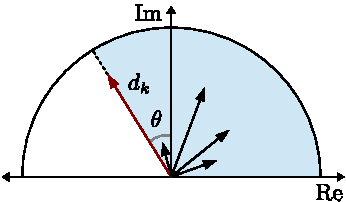
\includegraphics{fig/fig4.pdf}
%	\end{center}
%\caption{All demands lie in the shaded area. We measure $\theta = \phi - \frac{\pi}{2}$ from the imaginary axis.}
%	\label{f4}
%\end{figure}
 

We present a  $(1,1+\epsilon)$-approximation  for \textsc{CKP} denotee by Algorithm {\sc CKP-FPTAS} that is polynomial in both $\frac{1}{\epsilon}$ and $n$ (i.e., FPTAS). This algorithm is illustrated in a previous work~\cite{CEK14CKP}.

% We assume that $\tan \theta$ is bounded polynomial $P(n)\ge 1$ in $n$.
%; as we will see in the next section, without this assumption, a bi-criteria FPTAS is unlikely to exist. 

%Let $\cN_+\triangleq \{k \in \cN \mid d_k^{\rm R} \ge 0\}$ and $\cN_-\triangleq\{k \in \cN \mid d_k^{\rm R} < 0\}$ be the subsets of users with demands in the first and second quadrants respectively. Consider any  solution $S$ to \textsc{CKP$[0,\pi\mbox{-}\varepsilon]$} and define $S_+ \triangleq \{ k \mid d_k^{\rm R} \ge 0, k \in S \}$ and $S_- \triangleq \{ k \mid   d_k^{\rm R} < 0, k \in S \}$ as the subsets of users with demands having non-negative and negative real components respectively. 

The basic idea of Algorithm {\sc CKP-FPTAS} is to enumerate the guessed total projections on real and imaginary axes.% for $S_+^\ast$ and $S_-^\ast$ respectively. 
%We can use $\tan \theta$ to upper bound the total projections for any feasible subset $S$ as follows:
%\begin{align}
% \sum_{k \in S} d_k^{\rm I} \le C, \quad
% \sum_{k \in S_- } - d_k^{\rm R}   \le  C \tan \theta, \quad 
% \sum_{k \in S_+}  d_k^{\rm R}   &\le C(1+ \tan \theta). \label{eq:ubounds}
%\end{align}
We then solve two separate {\sc 2DKP} problems  to find subsets of demands that satisfy the individual guessed total projections. But since {\sc 2DKP} is generally NP-hard, we need to round-up the demands to get a problem that can be solved efficiently by dynamic programming. We show that the violation of the optimal solution to the rounded problem w.r.t. to the original problem is small in $\epsilon$. 

Next, we describe the rounding in detail. First, we define
%\footnote{For a more efficient procedure, we may replace $P(n)$ by $\max\{\tan \theta,1\}$; however, choosing $L$ to depend only on $P(n)$, and thus independent of the demands, will be needed for the truthful mechanism in Sec. \ref{sec:tbp}} 
$L \triangleq \frac{\epsilon C}{n}$, such that the new rounded-up demands $\hat{S_k}$ are defined by:
\begin{equation}
\hat S_k =
\hat S_k^{\rm R} + {\bf i} \hat S_k^{\rm I} \triangleq  
\left\lceil \frac{S_k^{\rm R}}{L} \right\rceil \cdot L + {\bf i} \left\lceil \frac{S_k^{\rm I}}{L} \right\rceil \cdot L
\label{eq:truc}
\end{equation}
Let $\xi$, $\zeta$  be respectively the guessed real and imaginary absolute total projections of the rounded demands in $S^\ast$.
%\begin{equation}
%\xi_+ \triangleq \{ d_k^{\rm R} \mid  k \in S_+ \}, \  \zeta_+ \triangleq \{ d_k^{\rm I} \mid  k \in S_+ \}, \ \xi_- \triangleq \{ - d_k^{\rm R} \mid  k \in S_- \}, \  \zeta_- \triangleq \{ %d_k^{\rm I} \mid  k \in S_- \}
%\end{equation}
Then the possible values of $\xi$ and $\zeta$ are integer mutiples of $L$:
\begin{align}
% \xi \in {\cal A}_+ & \triangleq \left\{0, L, 2L,\ldots,\left\lceil \frac{C (1 + P(n) )}{L} \right\rceil \cdot L\right\},\\
%\xi_- \in {\cal A}_- &\triangleq \left\{0,L, 2L,\ldots, \left\lceil \frac{C \cdot P(n) }{L} \right\rceil\cdot L \right\}, \nonumber \\
\xi, \zeta  \in {\cal A} & \triangleq \left\{0, L, 2L,\ldots,\left\lceil \frac{C}{L} \right\rceil\cdot L.\right\}
\label{eq:grid}
\end{align}
%Note that a feasible guess of total projections should satisfy constraint Eqn.~\raf{C1} for \textsc{CKP}, and thus:
%\begin{equation}\label{eq:sat}
%(\xi_+ - \xi_-)^2 + (\zeta_+ + \zeta_-)^2 \le (1+2\epsilon)^2C^2;
%\end{equation}
%see Lemma~\ref{lem-trunc} below. 
%Step \ref{alg:tight} forces the corresponding selected demands to be tight; otherwise, constraint Eqn.~\raf{C1} could be violated largely. Now, for each guess, we consider solving two {\sc 2DKP} instances separately. The first one with capacities $\xi_+$, $\zeta_+$ and positive demands $\hat d_k, k \in \cN_+$, and the second with $\xi_-,\zeta_-$ and demands in $\cN_-$. 


The next step is to solve the rounded instance exactly. Assume an arbitrary order on $\cN = \{ 1, ..., n\}$. We use recursion to define a 3D table, with each entry ${U}(k,c_1, c_2)$ as the maximum utility obtained from a subset of users $\{1,2,\dots,k\} \subseteq \cN$ with demands $\{\hat{S_1},\hat{S_2},...,\hat{S_k}\}$ that can fit exactly (i.e., satisfies the capacity constraint as an equation) within capacity $c_1$ on the real axis and $c_2$ on the imaginary axis. 

The cells are defined according to the following rules:
\begin{align}
{U}(1,C_1, C_2) &\triangleq  \left\{ \begin{array}{l l}
u_k & \quad \text{if $\hat{P_k} = C_1$ and $\hat Q_k  = C_2$}\\
-\infty &\quad \text{otherwise} \end{array}\right.\label{eq:dyn-rule1}\\
{U}(i+1,C_1, C_2) &\triangleq \max  \left\{ \begin{array}{l}
u_{i+1} + {U}(i, C_1 - \hat P_k, C_2 - \hat Q_k),\\
{U}(i,C_1,C_2)
 \end{array}\right.
 \label{eq:dyn-rule2}
\end{align}

%We denote by {\sc 2DKP-Exact}$[\cdot]$ the algorithm for solving {\sc 2DKP} by dynamic programming.


%\begin{algorithm}[!htb]
%\caption{{\sc CKP-FPTAS} $( \{u_k,d_k\}_{k \in \cN}, C,\epsilon) $}\label{CKP-FPTAS}
%\begin{algorithmic}[1]
%\Require Users' utilities and demands $\{u_k,d_k\}_{k\in \cN}$; capacity $C$; accuracy parameter $\epsilon$
%\Ensure $(1,1+3\epsilon)$-solution $\hat{S}$ to \textsc{CKP$[0,\pi\mbox{-}\varepsilon]$}
%\State $\hat{S} \leftarrow \varnothing$.
%\ForAll {$d_k$ and $k \in \cN$}
%\State Set $\hat d_k \leftarrow \hat d_k^{\rm R} + {\bf i} \hat d_k^{\rm I} $ as defined by \raf{eq:truc}
%\EndFor
%\ForAll {$\xi, \zeta  \in {\cal A}$}
%\If {$\xi^2 + \zeta^2 \le (1+2\epsilon)^2C^2$}\label{cond1}
%\State $ F \leftarrow \text{\sc 2DKP-Exact}(\{u_k,\frac{\hat d_k}{L}\}_{k\in\cN_+}, \frac{\xi}{L},\frac{\zeta}{L})$
%%\State $ F_- \leftarrow \text{\sc 2DKP-Exact}(\{u_k, \frac{-\hat d_k}{L}\}_{k\in \cN_-}, \frac{\xi_-}{L},\frac{\zeta_-}{L})$ 
%%\If{$F_+, F_- \neq \varnothing$} \label{alg:tight}
%\If{$u(F) > u (\hat{S})$}
%\State $\hat{S} \leftarrow  \{F\}$
%\EndIf 
%%\EndIf 
%\EndIf
%\EndFor
%\State \Return $\hat{S}$
%\end{algorithmic}
%\end{algorithm}


%\begin{algorithm}[!htb]
%\caption{{\sc 2DKP-Exact} $( \{u_k,\hat d_k\}_{k \in \cN'}, C_1,C_2) $}
%\begin{algorithmic}[1] 
%\Require Users' utilities and integer demands $\{u_k,\hat d_k\}_{k\in \cN'}$; integer capacities $C_1,C_2$
%\Ensure A utility-maximizing subset of satisfiable users $\subseteq \cN'$ subject to capacity constraints defined by $C_1,C_2$
%\State Create a 3D table of size $|\cN'| \times (C_1+1) \times (C_2+1)$, with each entry ${U}(k,c_1, c_2)$ according to: 
%\begin{align}
%{U}(1,c_1, c_2) &\triangleq  \left\{ \begin{array}{l l}
%u_1 & \quad \text{if $\hat d_1^{\rm R} = c_1$ and $\hat d_1^{\rm I}  = c_2$}\\
%-\infty &\quad \text{otherwise} \end{array}\right.\label{eq:dyn-rule1}\\
%U(k, 0, 0) &\triangleq 0\\
% U(k, c_1', c_2') &\triangleq -\infty\text{ for all }c_1'<0 \text{ or } c_2'<0\\
%{U}(k,c_1, c_2) &\triangleq \max  \Big\{ 
%u_{k} + {U}(k-1, c_1 - \hat d_k^{\rm R}, c_2 - \hat d_k^{\rm I}), \nonumber\\
%& \qquad \qquad {U}(k-1,c_1,c_2) \Big\}
% \label{eq:dyn-rule2}
%\end{align}
%\State Create a 3D table of size $|\cN'| \times C_1 \times C_2$, with each each entry ${\cI}(k,c_1, c_2)$ according to: 
%
%\begin{align}
%\cI(1,c_1, c_2) &\triangleq \left\{\begin{array}{l l}
%\{1 \}& \ \text{if $U(1,c_1,c_2) = u_1$}\\
%\varnothing & \ \text{otherwise} 
%\end{array}\right.\\
%%%%%%%%%%%%
%{\cI}(k,c_1, c_2) &\triangleq  \left\{ \begin{array}{ll}
%{\cI}(k-1,c_1, c_2) &\\
% \qquad \text{if ${U}(k,c_1, c_2) = {U}(k-1, c_1, c_2)$} \\
%%
%{\cI }(k-1,c_1- \hat d_k^{\rm R}, c_2- \hat d_k^{\rm I}) \cup \{ k \} \\
%  \qquad \text{if } {U}(k,c_1, c_2) = u_{k} + \\\qquad \qquad {U}(k-1, c_1 - \hat d_k^{\rm R}, c_2 - \hat d_k^{\rm I}) & \\
%\end{array}\right.
%%%%%%%%%%%
% \label{eq:dyn-rule3}
%\end{align}
%\State \Return $\displaystyle {\cI}(|\cN'|,C_1,C_2)$.
%\end{algorithmic}
%\end{algorithm}


\begin{theorem}\label{thm:bptas}
Algorithm {\sc CKP-FPTAS} is $(1,1+3\epsilon)$-approximation for \textsc{CKP$[0,\pi\mbox{-}\varepsilon]$} and its running time is polynomial in both $n$ and $\frac{1}{\epsilon}$.
\end{theorem}


\iffalse
\begin{proof}
First, the running time is proportional to the number of guesses, upper bounded by $O(\frac{1}{\epsilon^4} n^{4} P^6(n))$. For each guess, {\sc 2DKP-Exact} constructs a table of size at most $O(\frac{1}{\epsilon^2} n^3 P^4(n))$. Since we assumed $P(n)$ is polynomial in $n$, the total running time is polynomial in $n$ and $\frac{1}{\epsilon}$.

To show the approximation ratio of 1, we note {\sc CKP-FPTAS} enumerates over all possible rounded projections subject to the capacity constraint in {\sc CKP} and that {\sc 2DKP-Exact} returns the exact optimal solution for each rounded problem. In particular, by Lemma \ref{lem-trunc} one of the choices would be rounded projection for the optimum solution $S^\ast$.   
It remains to show that the violation of the returned solution is small in $\epsilon$. This is given in Lemma~\ref{lem-trunc2} below, which shows that the solution $\hat S$ to the rounded problem violates the capacity constraint by only a factor at most $(1+3\epsilon)$. 
\end{proof}

%In fact, $\epsilon$ is inversely proportional to $\theta$. The larger $\theta$ the smaller $\epsilon$ is required for maintaining the precision. This can be observed from Eqn.~\raf{lem1-p2}.

For any set $S\subseteq\cN$, let us write $D_+(S)\triangleq\sum_{k\in S_+}P_k$, $D_-(S)\triangleq\sum_{k\in S_-}-P_k$, $D_I(S)\triangleq\sum_{k\in S}Q_k$, $\hat D_+(S)\triangleq\sum_{k\in S_+} \hat P_k$, $\hat D_-(S)\triangleq\sum_{k\in S_-} -\hat P_k$, and $\hat D_I(S)\triangleq\sum_{k\in S}\hat Q_k$. Then by \raf{eq:truc} and the fact that $x \le t \lceil \frac{x}{t} \rceil  \le x + t$ for any $x,t$ such that $t>0$, we have 
\begin{eqnarray}\label{eq:bds}
&\max\{\hat D_+(S)-L|S|,0\}\le D_+(S)\le \hat D_+(S),~~~\max\{\hat D_-(S)-L|S|,0\}\le D_-(S)\le \hat D_-(S), \nonumber \\ & \max\{\hat D_I(S)-L|S|,0\}\le D_I(S)\le\hat D_I(S).
\end{eqnarray}

\begin{lemma}
For any optimal solution $S^*$ to \textsc{CKP$[0,\pi\mbox{-}\varepsilon]$}, $L\triangleq \frac{\epsilon C}{nP(n)}$ and $\epsilon> 0$, we have
\begin{equation}
 \left( \sum_{k \in S^*} \hat d_k^{\rm R} \right)^2 +  \left(\sum_{k \in S^*} \hat   d_k^{\rm I} \right)^2  \le C^2 ( 1 + 2\epsilon)^2 .
 \label{eq:lem}
\end{equation}
 \label{lem-trunc}
\end{lemma}
\begin{proof}
%First, we note that any optimal solution $S^*$ satisfies constraint Eqn.~\raf{C1}:
%\begin{equation}
%\left(\sum_{k\in S^*} d_k^{\rm R} \right)^2 + \left( \sum_{k \in S^* } d_k^{\rm I}\right)^2 \le C^2
%\label{eq:C1}
%\end{equation}


Using~\raf{eq:bds},
\begin{align}
\left( \sum_{k \in S^*} \hat d_k^{\rm R} \right)^2 +  \left(\sum_{k \in S^*} \hat d_k^{\rm I} \right)^2 &=\left(\hat D_+(S^*)- \hat D_-(S^*)\right)^2 +  \hat D_I^2(S^*)\nonumber\\
&=\hat D_+^2(S^*)+\hat D_-^2(S^*)-2\hat D_+(S^*)\hat D_-(S^*)+\hat D_I^2(S^*)\nonumber\\ 
&\le (D_+(S^*)+nL)^2+(D_-(S^*)+nL)^2-2D_+(S^*) D_-(S^*)+(D_I(S^*)+nL)^2\nonumber\\
&=(D_+(S^*)-D_-(S^*))^2+D_I^2(S^*)+2nL (D_+(S^*)+D_-(S^*)+D_I(S^*))+3n^2L^2\nonumber\\
&= \left(\sum_{k\in S^*} d_k^{\rm R} \right)^2 + \left(\sum_{k\in S^*} d_k^{\rm I}  \right)^2 +2nL\left(\sum_{k\in S^*}|d_k^{\rm R}|+\sum_{k\in S^*}d_k^{\rm I}\right)+3n^2L^2\nonumber\\
&\le C^2 + 4nL (P(n)+1) C + 3n^2L^2 = C^2 + 4 \epsilon C^2 + 3\epsilon^2 C^2/(1+P(n))^2\nonumber \\ &\le C^2 (1+4\epsilon + \epsilon^2)\le C^2(1+2\epsilon)^2\label{lem1-p2}.
\end{align}
\end{proof}

\begin{lemma}\label{lem-trunc2}
Let $\hat S$ be the solution returned by {\sc CKP-FPTAS}. Then $|\sum_{k\in\hat S}d_k|\le(1+3\epsilon) C$. 
\end{lemma}
\begin{proof}
As in~\raf{lem1-p2},
\begin{align}\label{eq:ee1}
\left( \sum_{k \in \hat S} d_k^{\rm R} \right)^2 +  \left(\sum_{k \in \hat S} d_k^{\rm I} \right)^2 &=\left(D_+(\hat S)- D_-(\hat S)\right)^2 +  D_I^2(\hat S)\nonumber\\
&=D_+^2(\hat S)+D_-^2(\hat S)-2D_+(\hat S)D_-(\hat S)+D_I^2(\hat S).
\end{align} 
If both $\hat D_+(\hat S)$ and $\hat D_-(\hat S)$  are less than $nL$, then the R.H.S. of \raf{eq:ee1} can be bounded by 
\begin{align}\label{eq:ee2}
&\hat D_+^2(\hat S)+\hat D_-^2(\hat S)+\hat D_I^2(\hat S)
\le\hat D_+^2(\hat S)+\hat D_-^2(\hat S)-2\hat D_+(\hat S)\hat D_-(\hat S)+2n^2L^2+\hat D_I^2(\hat S)\nonumber\\
&=(\hat D_+(\hat S)-\hat D_-(\hat S))^2+\hat D_I^2(\hat S)+2n^2L^2.
\end{align}
Otherwise, we bound the R.H.S. of \raf{eq:ee1} by
\begin{align}\label{eq:ee3}
&\hat D_+^2(\hat S)+\hat D_-^2(\hat S)-2(\hat D_+(\hat S)-nL)(\hat D_-(\hat S)-nL)+\hat D_I^2(\hat S)\nonumber\\
&=(\hat D_+(\hat S)-\hat D_-(\hat S))^2+\hat D_I^2(\hat S)+2nL(\hat D_+(\hat S)+\hat D_-(\hat S))-2n^2L^2.
\end{align}
Since $\hat S=F_+\cup F_-$ is obtained from feasible solutions $F_+$ and $F_-$ to $\text{\sc 2DKP-Exact}(\{u_k,\hat d_k/L\}_{k\in\cN_+}, \xi_+/L,\zeta_+/L)$
 and $\text{\sc 2DKP-Exact}(\{u_k,-\hat d_k/L\}_{k\in \cN_-}, \xi_-/L,\zeta_-/L)$, respectively, and  $\xi_+ , \xi_-,\zeta_+, \zeta_-$ satisfy the condition in Step~\ref{cond1}, it follows from \raf{eq:ee1}-\raf{eq:ee3} that
\begin{align*}
\left( \sum_{k \in \hat S} d_k^{\rm R} \right)^2 +  \left(\sum_{k \in \hat S} d_k^{\rm I} \right)^2 &\le \left( \sum_{k \in \hat S} \hat d_k^{\rm R}\right)^2 +  \left(\sum_{k \in \hat S}\hat d_k^{\rm I} \right)^2+2nL\sum_{k \in \hat S_-} |\hat d_k^{\rm R}|+2n^2L^2\nonumber\\
&=(\xi_+ - \xi_-)^2 + (\zeta_+ + \zeta_-)^2 + 2nL\xi_-+2n^2L^2\nonumber\\
&\le \left((1+2\epsilon)^2C^2 +2n\frac{\epsilon}{n(P(n)+1)} C^2 + 2n^2\frac{\epsilon^2}{n^2(P(n)+1)^2}\right)C^2\\
&\le \left((1+2\epsilon)^2 +\epsilon + \frac{\epsilon^2}{2}\right)C^2\le (1+3\epsilon)^2C^2.
\end{align*}
\end{proof}

\iffalse
\begin{corollary}
For any $(\alpha, \beta)$-approximation algorithm of \textsc{CKP$[0,\pi\mbox{-}\varepsilon]$} using truncated demands $\hat d_k$, we have $(\alpha, \beta (1+\epsilon))$-approximation for original demands $d_k$.
\label{cor} 
\end{corollary}
This follows immediately from Lemma~\ref{lem-trunc}. The approximation ratio $\alpha$ remains the same since any optimal $S^*$ is also feasible in the new instance within a violation of $(1+\epsilon)$.
\fi

\fi
